\section{Propulsion} \label{sec:prop}

Thrust is provided by a SRAD pressure fed bi-propellant liquid propulsion system. It utilizes nitrous oxide and ethanol as propellants and is pressurized by two nitrogen tanks through mechanical pressure regulators. The system is optimized for simplicity, low mass and small size. It can roughly be divided into three main subsystems which are described in detail below: the propellant tanks with piping, the pressurization systems and the engine with its valves and fill connections. A diagram of the whole fluid system, including the connected ground systems, can be found in \Cref{sec:sysarch_fluidSystem}.

The entire propulsion system, which is shown in \Cref{fig:sysarch_prop_propSystem} is assembled separately from the rest of the vehicle and can be tested standalone without it. It is installed into the airframe by sliding it into the body tube from the rear as one integrated component, only requiring two electrical connectors to be plugged in and a few screws to be installed.

\begin{figure}[H]
\centering
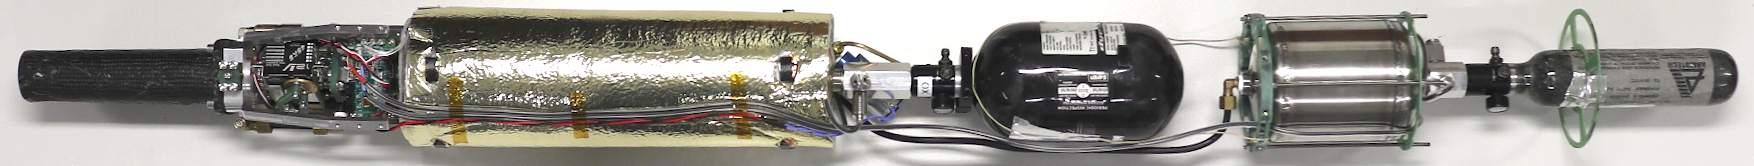
\includegraphics[width=\textwidth]{Propulsion/propSystem.png}
\caption{Complete propulsion system, ready to be installed into the airframe}
\label{fig:sysarch_prop_propSystem}
\end{figure}

\subsection{General Parameters}

The thrust is chosen to be \SI{600}{\newton} at liftoff as a trade-off between sufficient launch acceleration for aerodynamic stability and the capacity of the engine testing infrastructure. The chamber pressure and oxidizer/fuel mass flow ratio (O/F ratio) is chosen as a trade off between engine efficiency, combustion temperature, propellant mass flows and feed pressures.
As a compromise between high efficiency, low heat transfer into the thrust chamber and low feed pressures, a chamber pressure of \SI{15}{\bar} is chosen. \Cref{fig:sysarch_engPerf} shows various engine parameters as a function of the O/F ratio.

\begin{figure}[H]
\centering
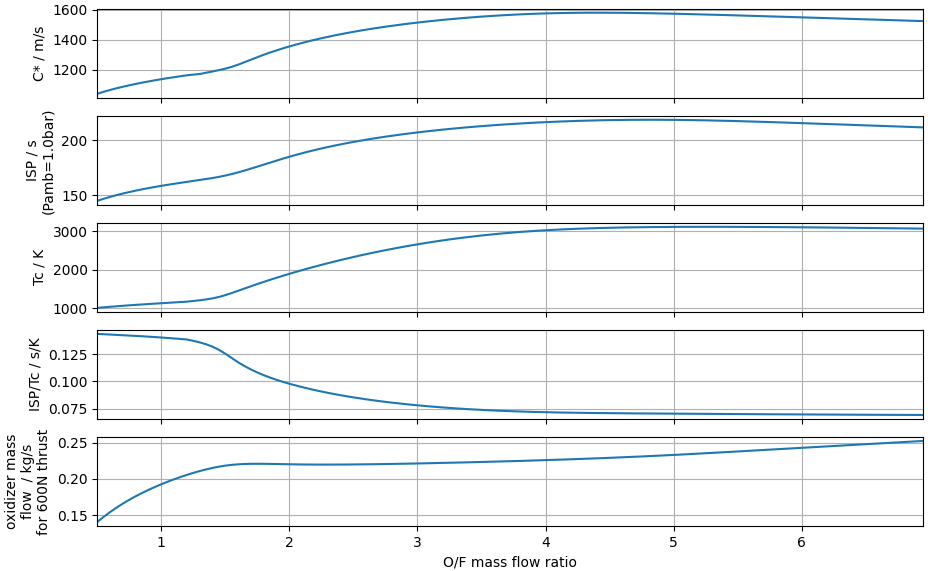
\includegraphics[width=\textwidth]{Propulsion/engineParameters.png}
\caption{Ideal engine performance parameters as a function of the oxidizer/fuel mass flow ratio at a chamber pressure of \SI{15}{\bar}}
\label{fig:sysarch_engPerf}
\end{figure}

Since the oxidizer mass flow rate is nearly constant at ratios above 1.5 and smaller ratios lead to unacceptable efficiency, this metric can be ignored. The fuel mass flow rate is not plotted but favors high ratios. The efficiency to combustion temperature ratio is highest at low O/F ratios but the efficiency is estimated to impact the vehicle mass more than the combustion temperature so a higher mass flow ratio of 3.0 is chosen based on this data.

As the vehicle will not reach high altitudes, the expansion ratio is sized for an ambient air pressure of \SI{1000}{\milli\bar}.
When assuming a \SI{93}{\percent} C* and ISP efficiency (based on previous engine testing data) and a thrust of \SI{600}{\newton}, the following engine parameters were calculated using the self developed Python program ORLEG \cite{orleg} which uses the CEA \cite{CEA} Python wrapper RocketCEA \cite{RocketCEA}:

\begin{itemize}
\item throat diameter: \SI{19}{\milli\meter}
\item nozzle exit diameter: \SI{32}{\milli\meter}
\item nozzle expansion ratio: 2.7
\item combustion temperature: \SI{2632}{\kelvin}
\item c*: \SI{1405}{\meter\per\second}
\item ISP: \SI{192}{\second}
\item total mass flow rate: \SI{318}{\gram\per\second}
\item fuel mass flow rate: \SI{79}{\gram\per\second}
\item oxidizer mass flow rate: \SI{238}{\gram\per\second}
\end{itemize}

Considering the complete vehicle design, a burn time of about \SI{8}{\second} is necessary to reach the intended target altitude of \SI{3}{\kilo\meter}. The fuel tank is sized to a volume of \SI{900}{\milli\liter} and the oxidizer tank to \SI{2400}{\milli\liter}, fitting about \SI{700}{\gram} of fuel at ambient temperature and \SI{2085}{\gram} of oxidizer at a temperature of \SI{0}{\celsius} (see \cref{sec:sysarch_prop_oxLoad}) and an assumed fill level of 95\% due to boil-off between filling and launch. This gives a maximum burn time of up to \SI{8.8}{\second}, when a constant thrust of \SI{600}{\newton} is assumed. As the tank pressures and therefore mass flow rates and thrust drop off during the burn due to non-ideal pressure regulators, the burn time increases slightly.

\subsection{Propellant Tanks and Piping}

\begin{figure}[H]
\centering
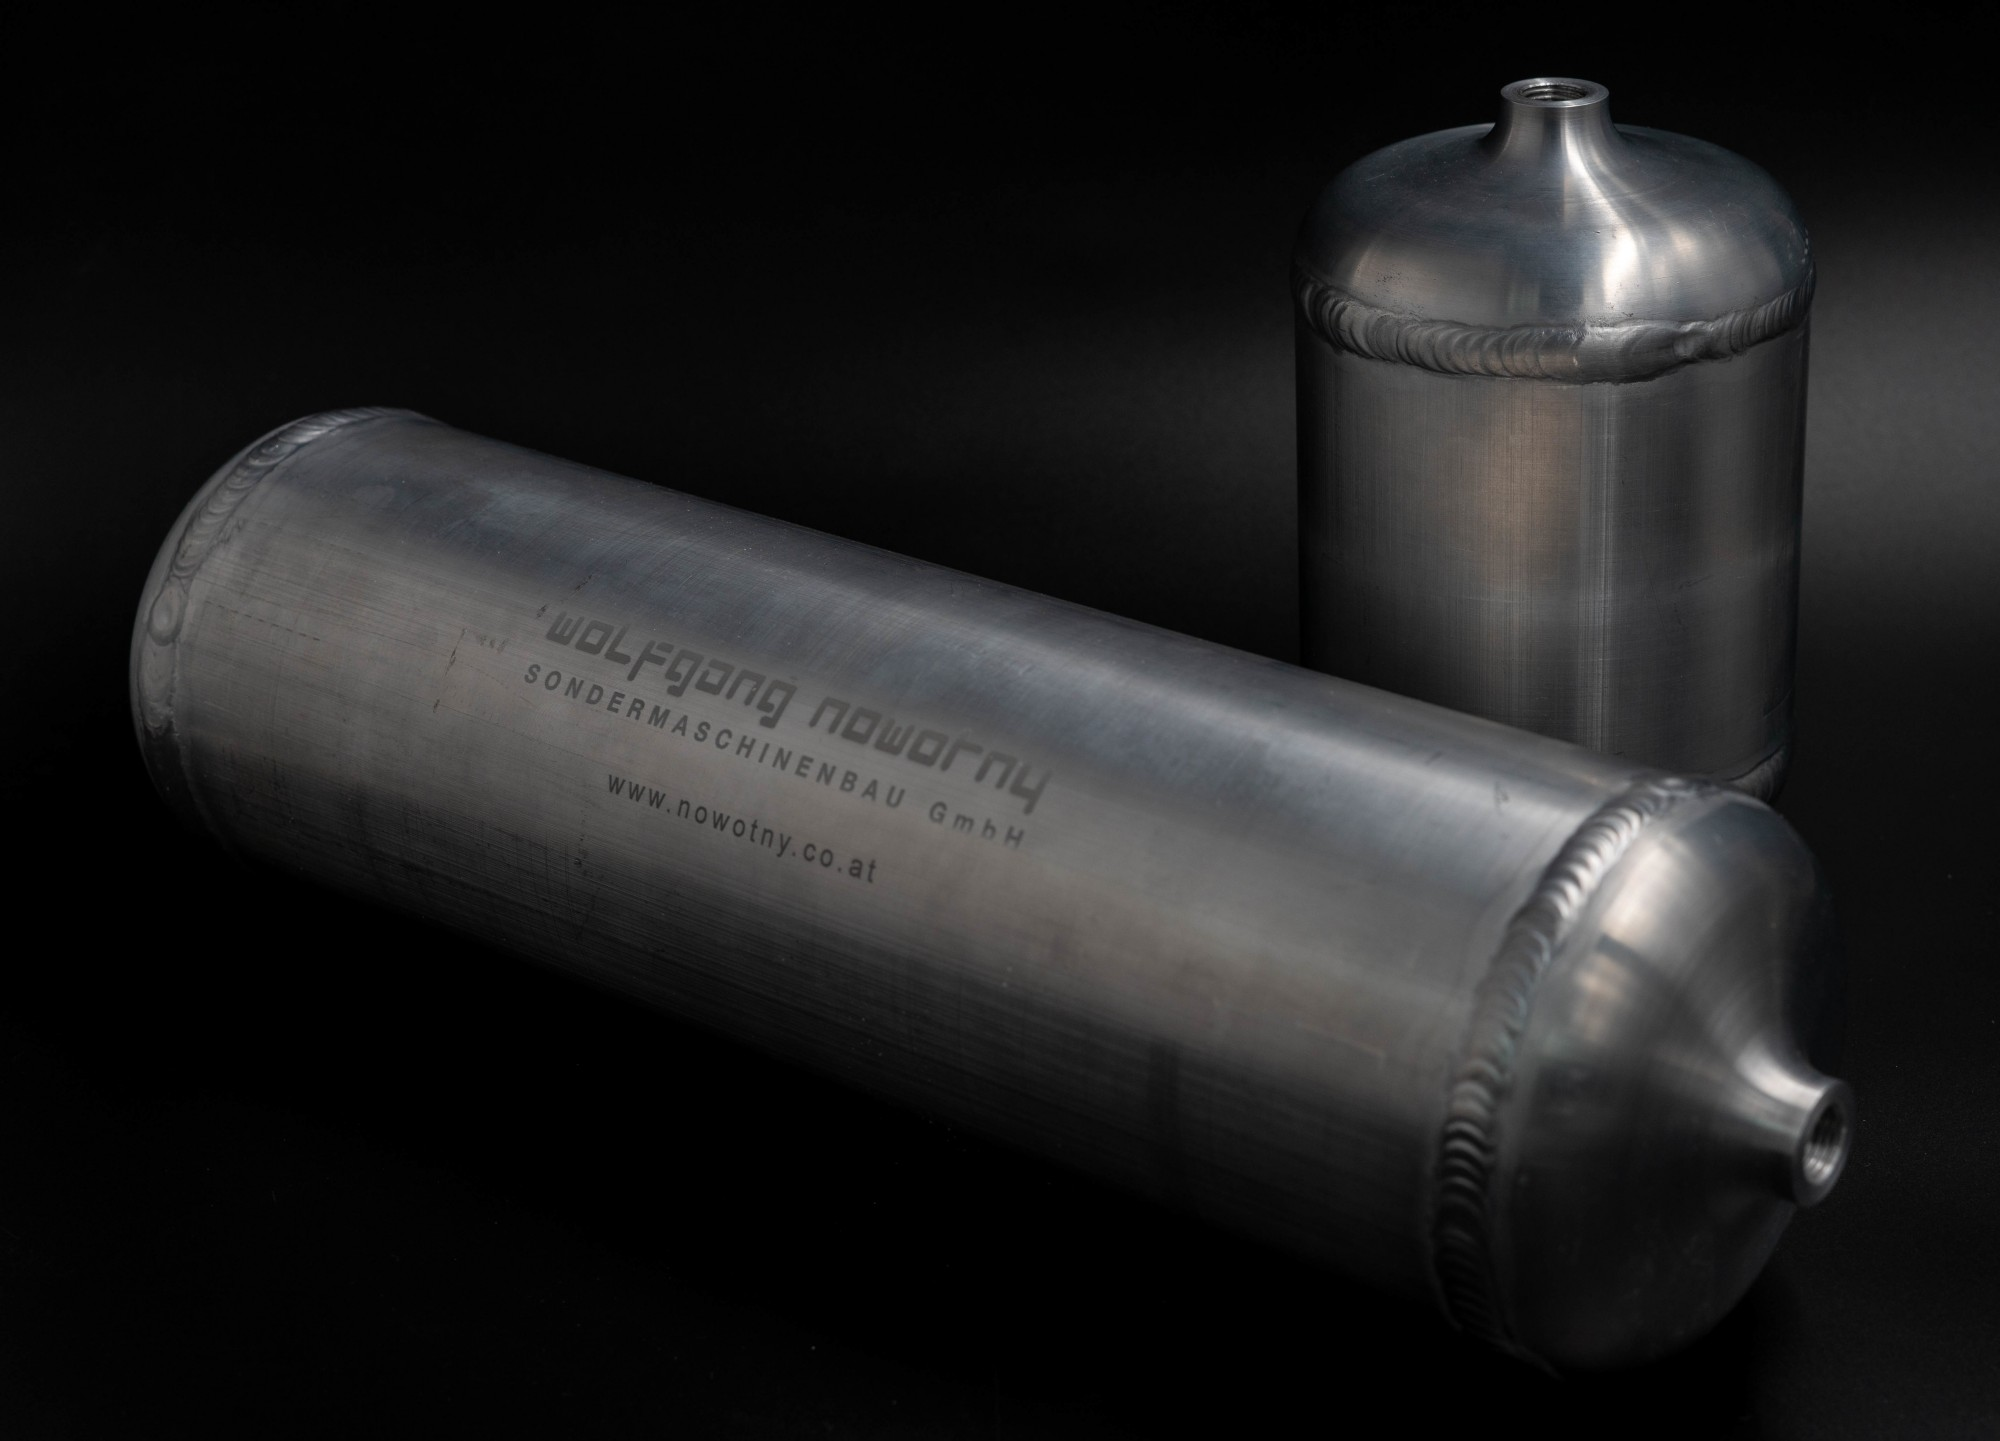
\includegraphics[width=\textwidth]{Propulsion/propTanks.jpg}
\caption{Aluminium propellant tanks}
\label{fig:sysarch_prop_propTanks}
\end{figure}

The propellant tanks, shown in \Cref{fig:sysarch_prop_propTanks} are manufactured from aluminium in three parts each that are welded together, the two end-caps with threaded connections and a tube in between. They were designed by the team but are one of the few components manufactured externally. This allowed for a more optimized end-cap design to be manufactured and additionally the welds were done by a professional welder, assuring consistency.

Sharing the end-cap design, the fuel and oxidizer tanks have a diameter of \SI{101}{\milli\meter}. A length of \SI{192}{\milli\meter} for fuel and \SI{387}{\milli\meter} for oxidizer gives the tanks a volume of \SI{900}{\milli\liter} and  \SI{2400}{\milli\liter} and a mass of \SI{594}{\gram} and \SI{1170}{\gram}.

To minimize mass, a heat treated high strength aluminium alloy is used, which at the same time has to be weldable. The choice fell on EN AW-6082. As there were uncertainties regarding the strength of the welded joints, which is crucial for this application, representative samples of the material were cut in half and welded back together by the designated tank manufacturer using the process planned for the tanks. After heat treatment for hardening, the samples were professionally tested for tensile strength, yielding good results. Based on those, the tanks were designed for a burst pressure of \SI{125}{\bar} and manufactured before receiving the same heat treatment as the samples.

The maximum nominal operating pressure of the tanks is about \SI{50}{\bar} for oxidizer and \SI{40}{\bar} for fuel. As under some circumstances, the tanks could be exposed to up to the \SI{60}{\bar} set pressure of the safety valves, the pressure used for proof testing was based on this value. With a 50\% safety factor, the tanks were hydrostatically tested at \SI{90}{\bar} for an extended amount of time, without showing leaks or other abnormalities. The detailed test report can be found in \Cref{sec:app_proof_pressure_testing}.

The oxidizer tank is axially supported by its connection to the engine assembly via the oxidizer tube and in turn axially supports the oxidizer pressurant system. Radial support against the body tube is provided by 3D-printed plastic spacers. As the pressurant fill connection needs to be aligned with the other fill connections, the connection between the oxidizer tube and the oxidizer valve (which is rigidly mounted to the engine) can be mounted with arbitrary rotation, as described in \Cref{sec:sysarch_prop_mainvalves}. To reduce heat flow into the tank, which causes the liquid oxidizer to boil off, the tank is wrapped in thermal insulation.

\begin{figure}[H]
\centering
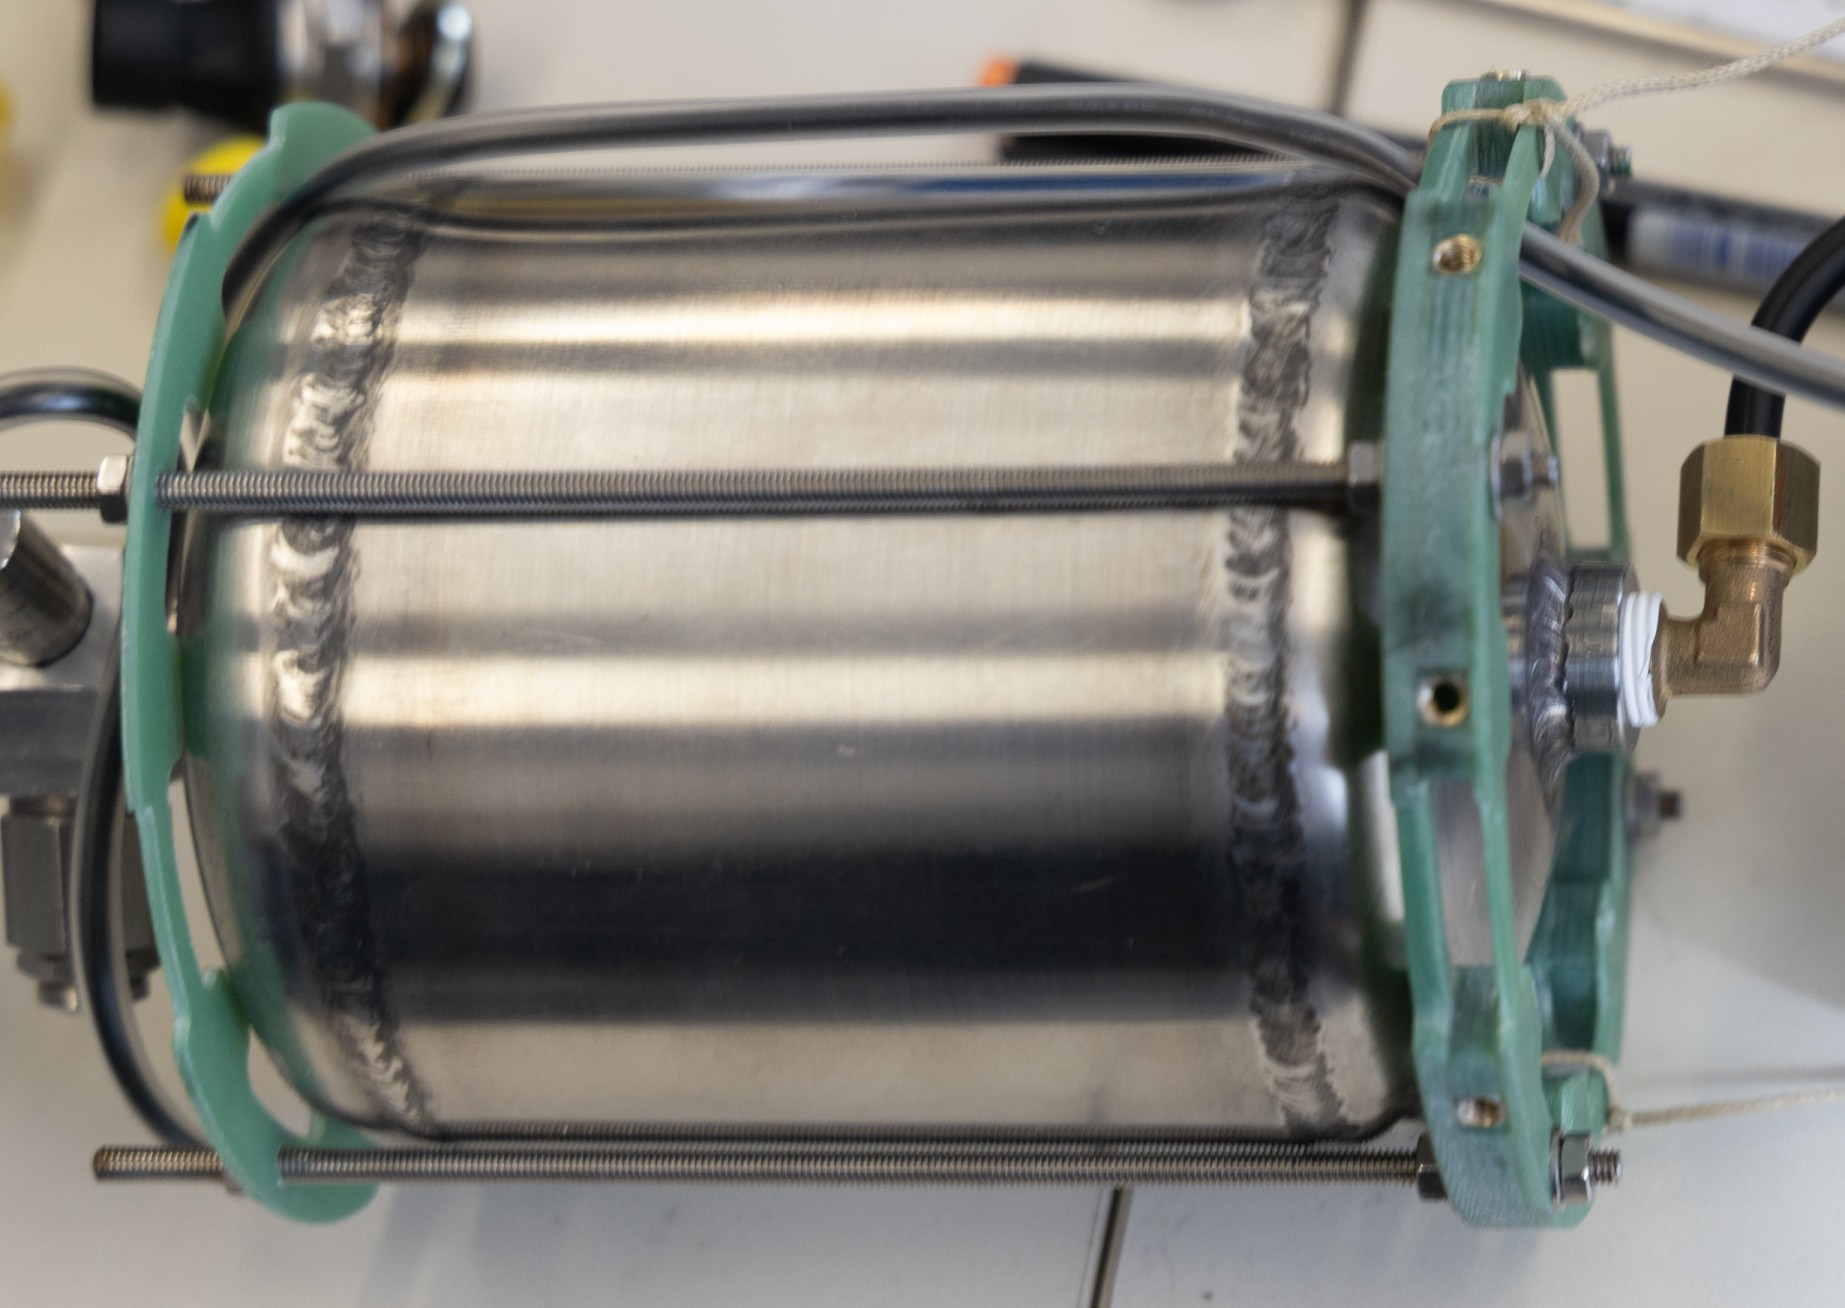
\includegraphics[width=0.7\textwidth]{Propulsion/fuelTankMounting.jpg}
\caption{Steel Prototype Fuel Tank in its mounting cage}
\label{fig:sysarch_prop_fuelTankMounting}
\end{figure}

The fuel tank also supports the fuel pressurization system but it is not rigidly connected to the rest of the propulsion system. Instead, the fuel tank is clamped in a cage made of GFRP plates and threaded rods (shown in \Cref{fig:sysarch_prop_fuelTankMounting}), which in turn is attached to the body tube via radial screws. During installation of the propulsion system into the body tube from the rear, the fuel system is pushed in by the rest of the propulsion system. It can then be manipulated from the front to seat the radial screws. As the fuel tank can be rotated within its mounting cage with a bit of force, the fuel systems rotation can then be finely adjusted to align the pressurant fill connection with the associated opening in the body tube. While the process may sound tedious, it is actually pretty simple and quick. To avoid the fuel system getting pulled out by the flexible fuel tube connecting it to the engine when pulling out the propulsion system, a piece of string connects the two subsystems and removes any tension from the fuel tube.

The connection between the fuel tank and engine is made with an aluminium-poliamide composite tube with an outside diameter of \SI{6}{\milli\meter} and a wall thickness of \SI{1}{\milli\meter}. It is flexible, light weight and compatible with standard compression ring fittings, making it well suited for this application. While the pressure rating given by the manufacturer is not sufficient for the application, it is given with a higher than needed safety factor, and the tube was successfully pressure tested to twice its maximum operating pressure.

\subsection{Pressurization System}

The fuel and oxidizer tanks are pressurized by nitrogen from two COPVs via mechanical pressure regulators. The COPVs with max. pressure of \SI{300}{\bar} and volumes of \SI{800}{\milli\liter} and \SI{250}{\milli\liter} for the fuel and oxidizer systems as well as the pressure regulators are COTS components, originally intended for pressurizing Paintball equipment.

The regulators exhibit less than ideal performance, with the fuel pressure dropping from \SI{40}{\bar} static pressure to \SI{30}{\bar} at startup due to the mass flow demand and then progressively down to \SI{25}{\bar} during the burn due to decreasing pressurant tank pressure. The oxidizer regulator behaves similarly with a pressure drop from \SI{50}{\bar} static to \SI{40}{\bar} at startup and down to \SI{35}{\bar} during the burn.
While this behaviour is far from ideal and additionally varies a bit from run to run, it is good enough for this vehicle.
The additional influence of the acceleration on the pressure differential between the top of the propellant tanks and the injector can be ignored due to the vehicles small size.

Active pressure control using electrically actuated valves and a software control loop was evaluated with good preliminary results but got abandoned in favor of the simple solution using mechanical regulators. For larger vehicles or more stringent pressure accuracy requirements, active control would be the preferred method though.

No pressurization valves are used, so the propellant tanks get pressurized as soon as the pressurant tanks get filled (the regulators include fill connections and check valves), which (apart from a partial pre-pressurization before oxidizer filling) only happens shortly before liftoff, see \Cref{sec:prop_pressfill}.

\begin{figure}[H]
\centering
\subfloat[Fuel]{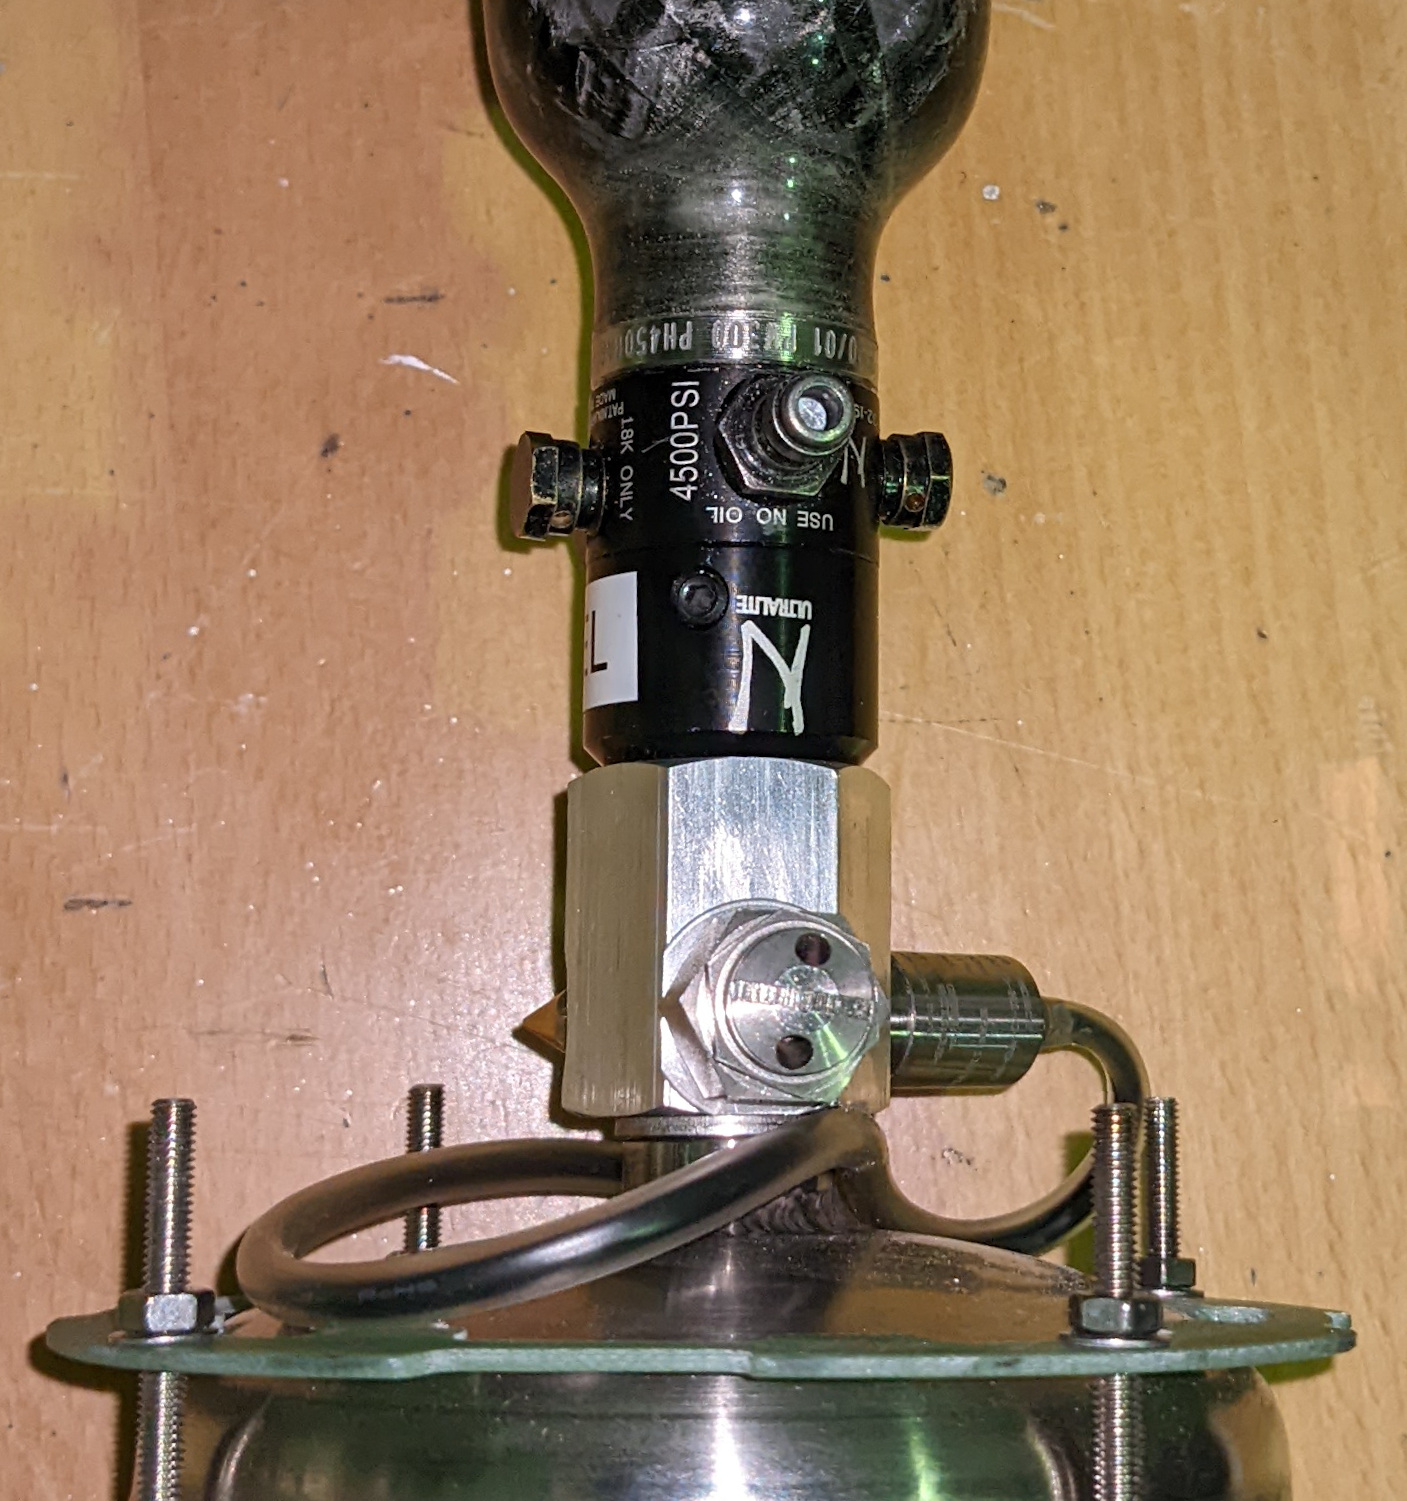
\includegraphics[width=0.3\textwidth]{Propulsion/fuelManifold.jpg}}
\subfloat[Oxidizer]{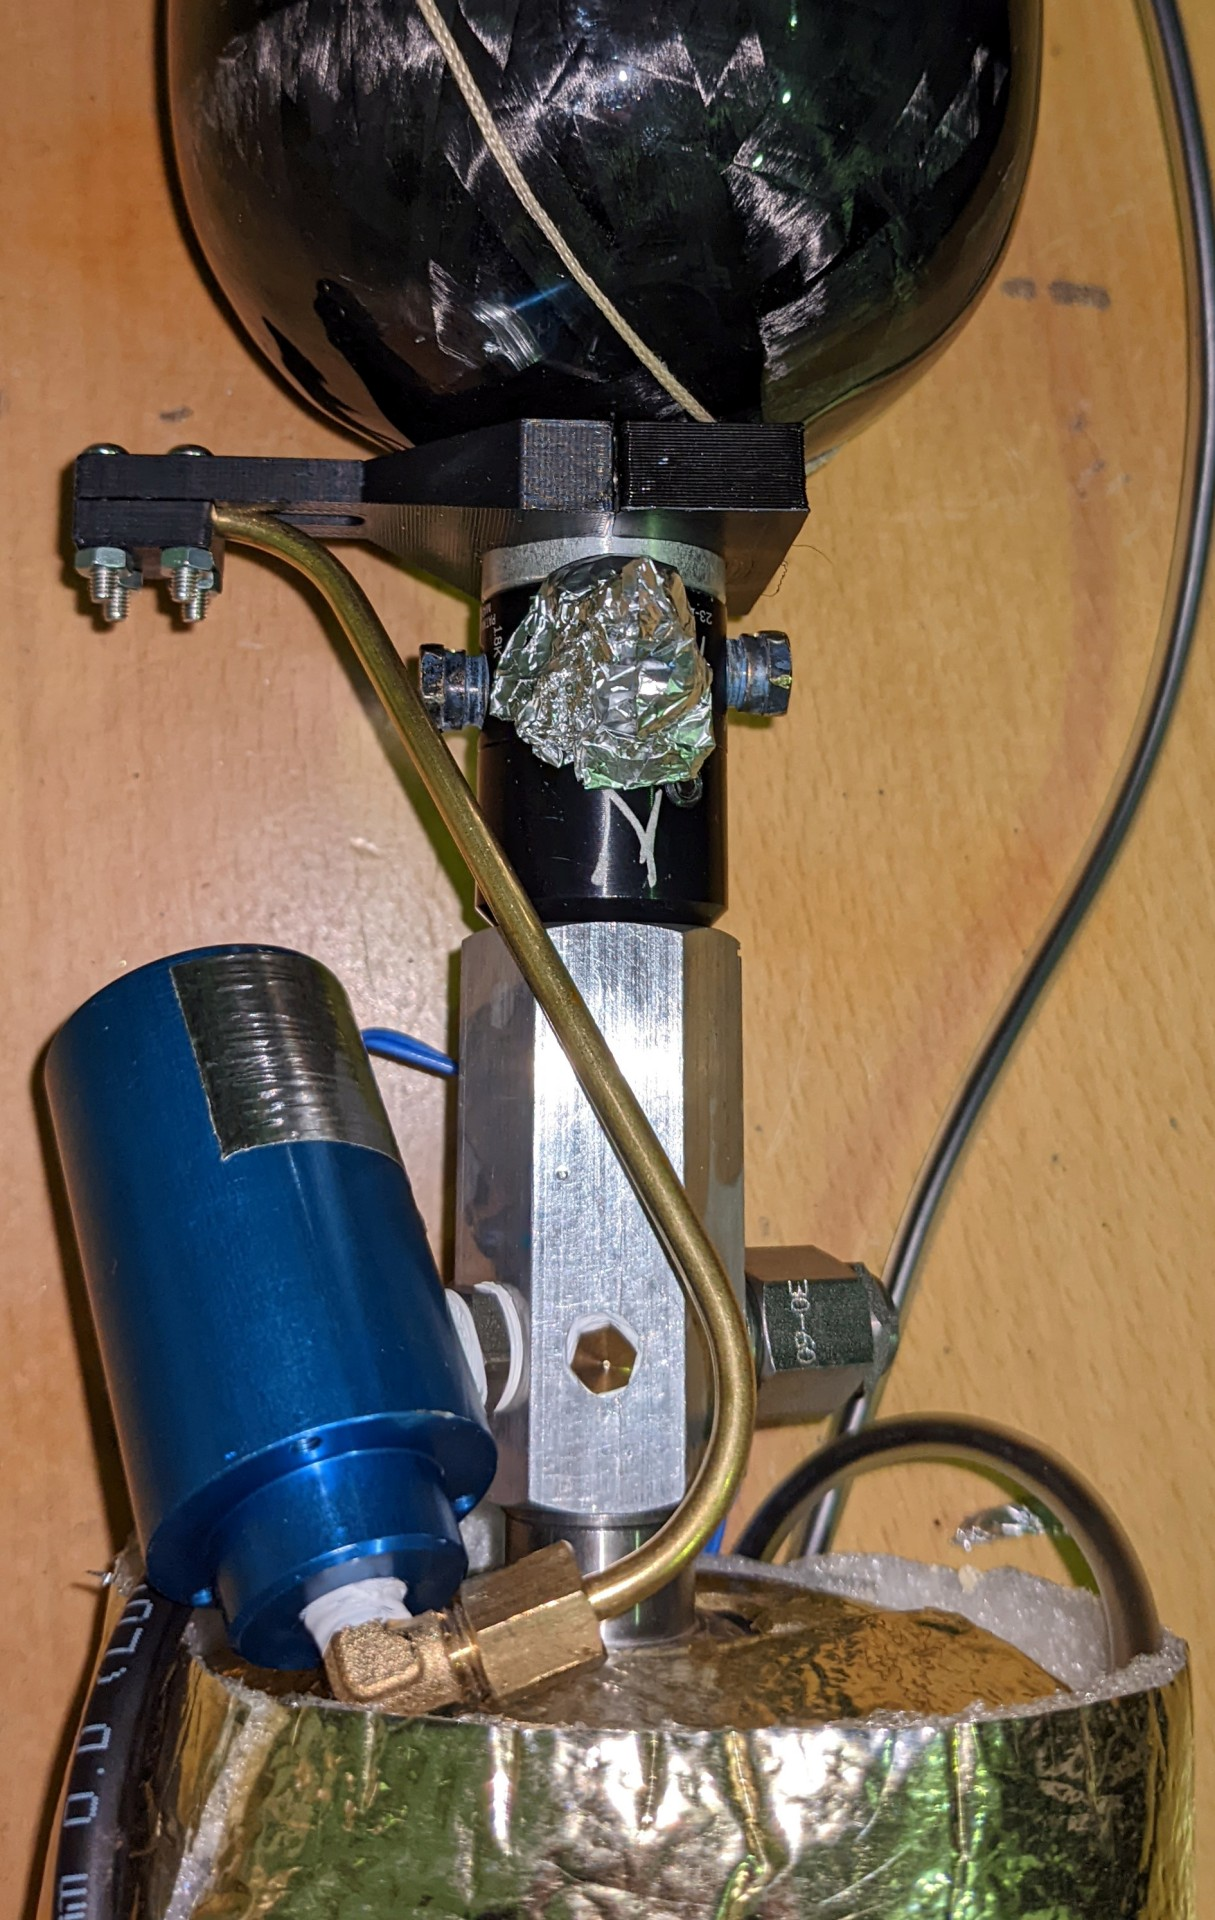
\includegraphics[width=0.3\textwidth]{Propulsion/oxManifold.jpg}}
\subfloat[Oxidizer]{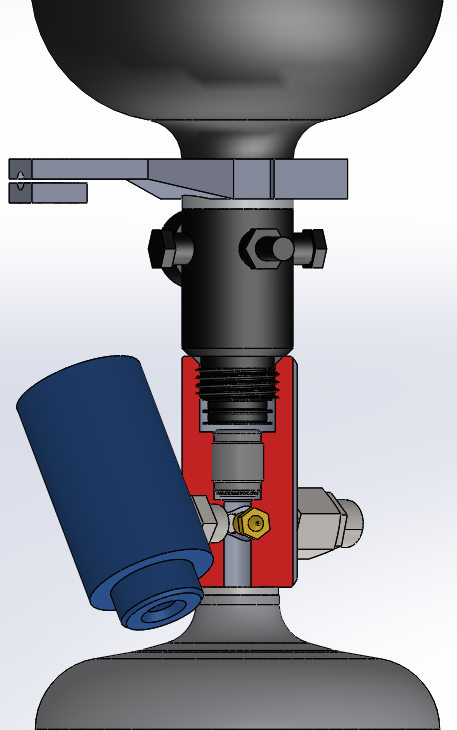
\includegraphics[width=0.3\textwidth]{Propulsion/oxManifoldCut.png}}
\caption{Pressurization manifolds with connected components}
\label{fig:sysarch_prop_pressManifolds}
\end{figure}

The output sides of the pressure regulators are screwed into the top of aluminium manifolds, which connects multiple components together. In case of the oxidizer, an inline check valve is integrated inside the manifold after the regulator to prevent any oxidizer flowing back into the pressurization system, this is not needed for the fuel side. The bottom side of the manifolds is screwed into the top of the propellant tanks. Connected on the sides of each manifold are a tank pressure sensor, a safety valve and a bleed orifice. The assemblies are shown in \cref{fig:sysarch_prop_pressManifolds}.

The safety valves are set to their maximum of \SI{60}{\bar}, well under the tanks proof and burst pressures. The bleed orifice consists of a \SI{0.1}{\milli\meter} 3D-printing nozzle that is used to slowly depressurize the system over time. This helps to safe the vehicle in case of a complete avionics failure and does not negatively impact normal operations. 

On the oxidizer manifold, a solenoid vent valve is installed as well, to allow for active regulation of the tank pressure and thus oxidizer temperature during and after filling, see \Cref{sec:sysarch_prop_oxLoad}. The output of the solenoid valve flows through a tube to an opening in the body tube, to not cause pressure spikes within the airframe that could trigger the recovery electronics, and to make the vented plume visible, which helps recognize the completion of the filling process.

The regulators include two burst discs, one with a \SI{517}{\bar} burst pressure to protect the pressurant bottle and one with a \SI{124}{\bar} burst pressure on the output. Since this output burst disc's burst pressure is much greater than the opening pressure of the safety valves, this burst disc is not expected to be needed unless the safety valves fail and an overpressure event is caused. In case of the oxidizer system, the burst disc can only protect against overpressure caused by a regulator failure, as overpressure originating from the oxidizer tank can't flow back to the burst disc through the check valve.

Both pressurization system assemblies are axially supported by the connection to their respective propellant tank. Radial support against the body tube for the pressurant tanks is provided by a GFRP spacer plate for the fuel tank and 3D-printed plastic spacers for the oxidizer tank.

\subsection{Engine, Valves and Fill Connections}
\label{sec:engine_valves_fill_connections}

\begin{figure}[H]
\centering
\subfloat{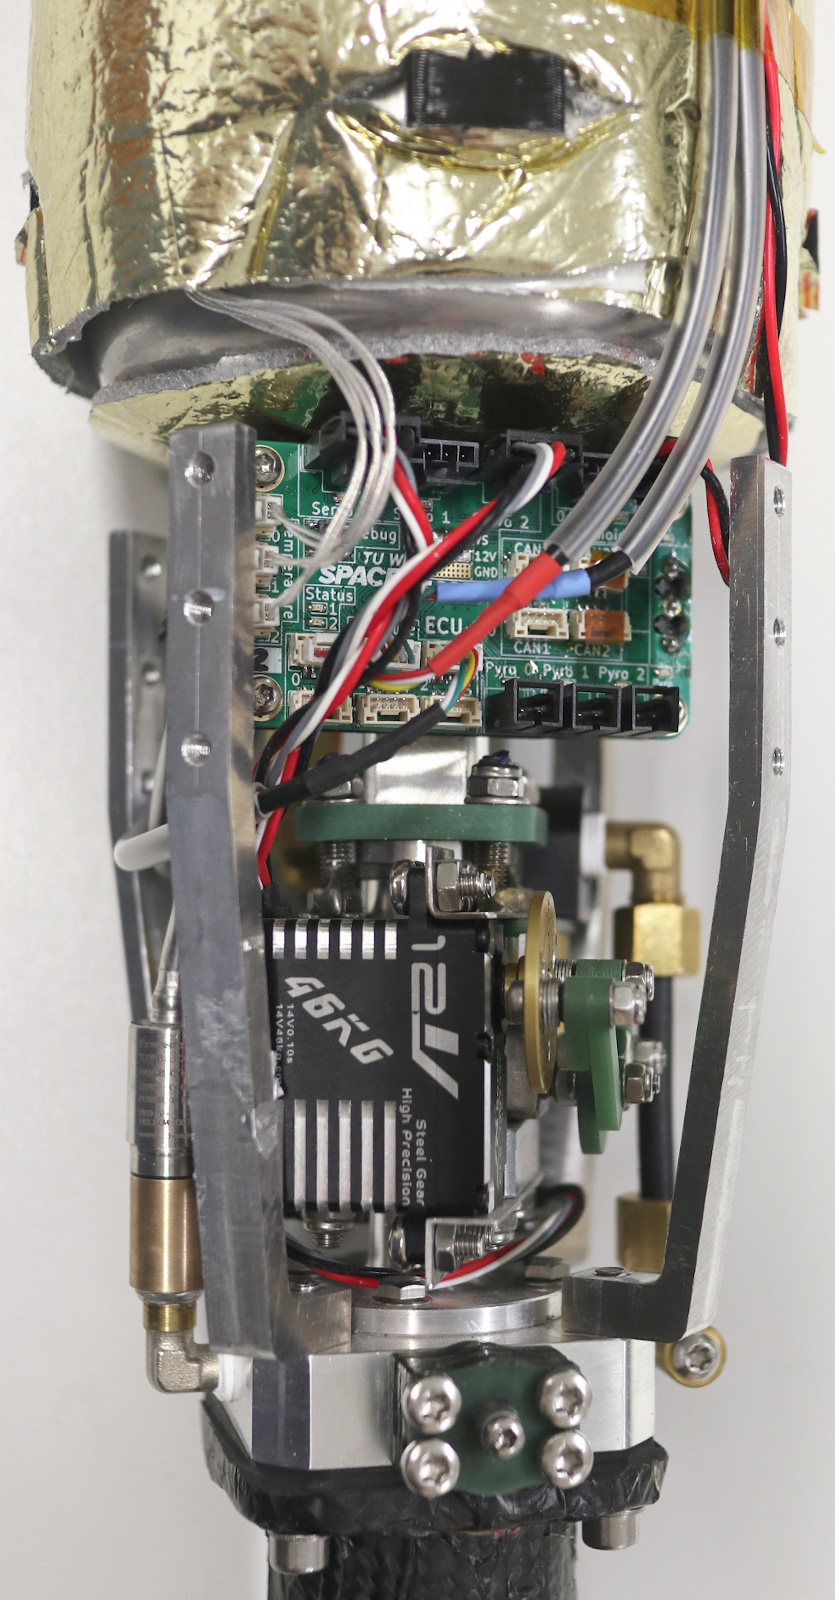
\includegraphics[width=0.25\textwidth]{Propulsion/engineAssy_1.jpg}}
\subfloat{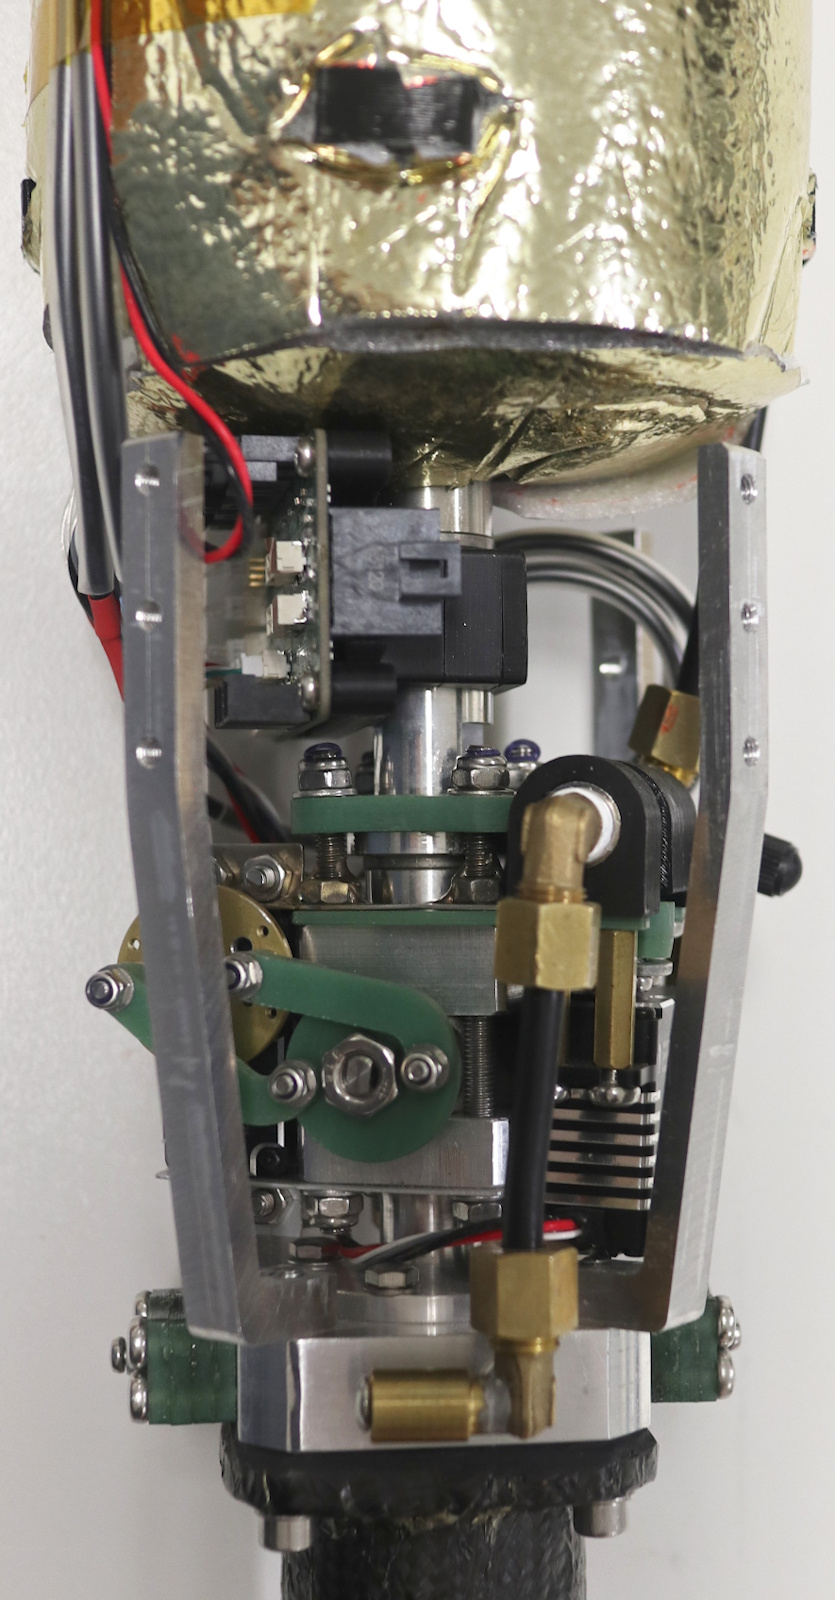
\includegraphics[width=0.25\textwidth]{Propulsion/engineAssy_2.jpg}}
\subfloat{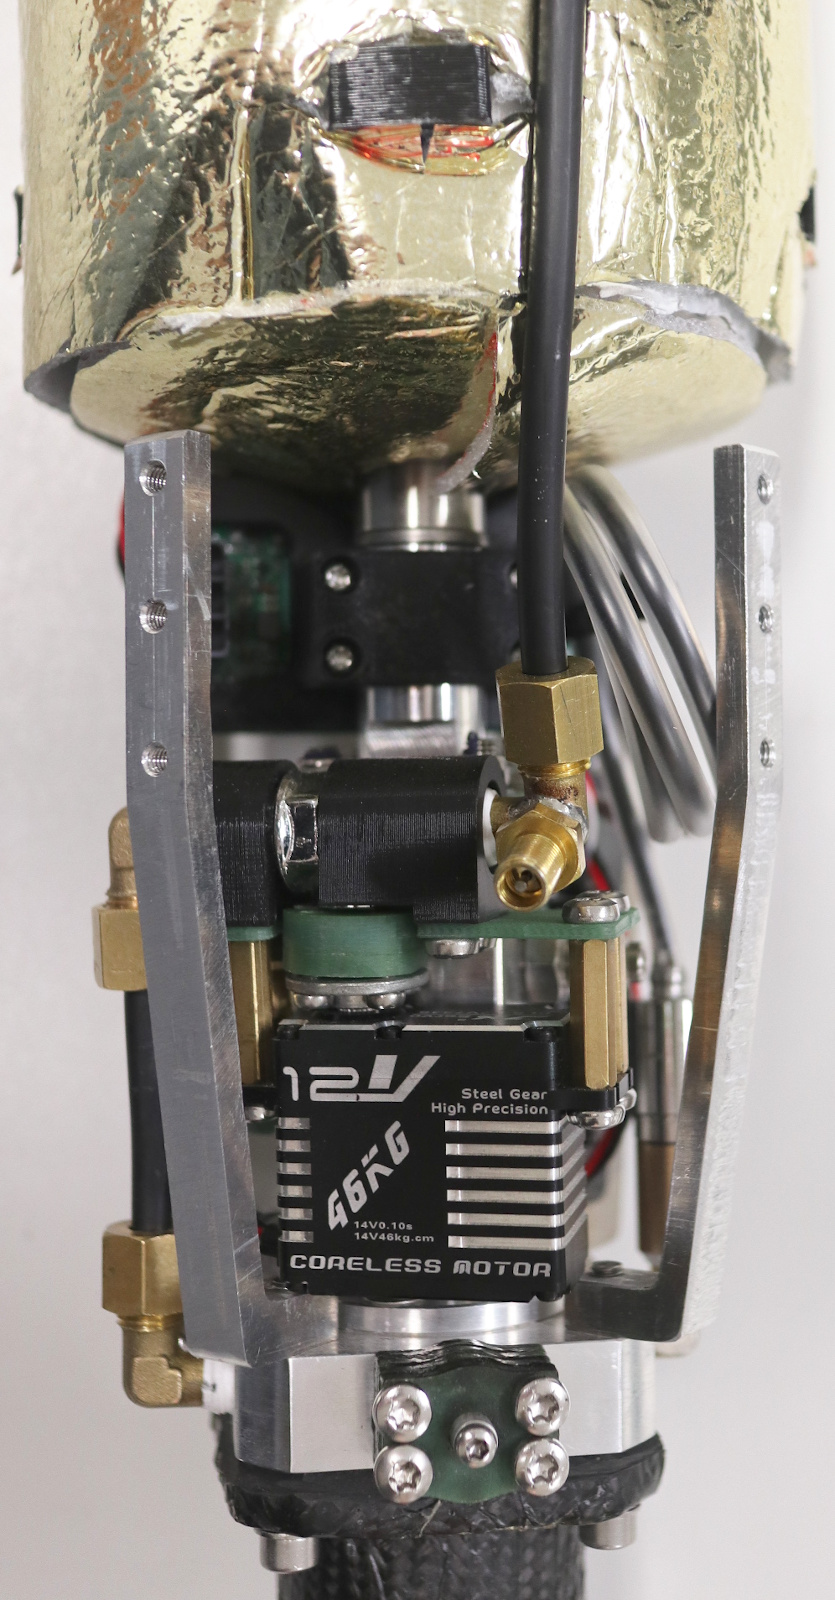
\includegraphics[width=0.25\textwidth]{Propulsion/engineAssy_3.jpg}}
\subfloat{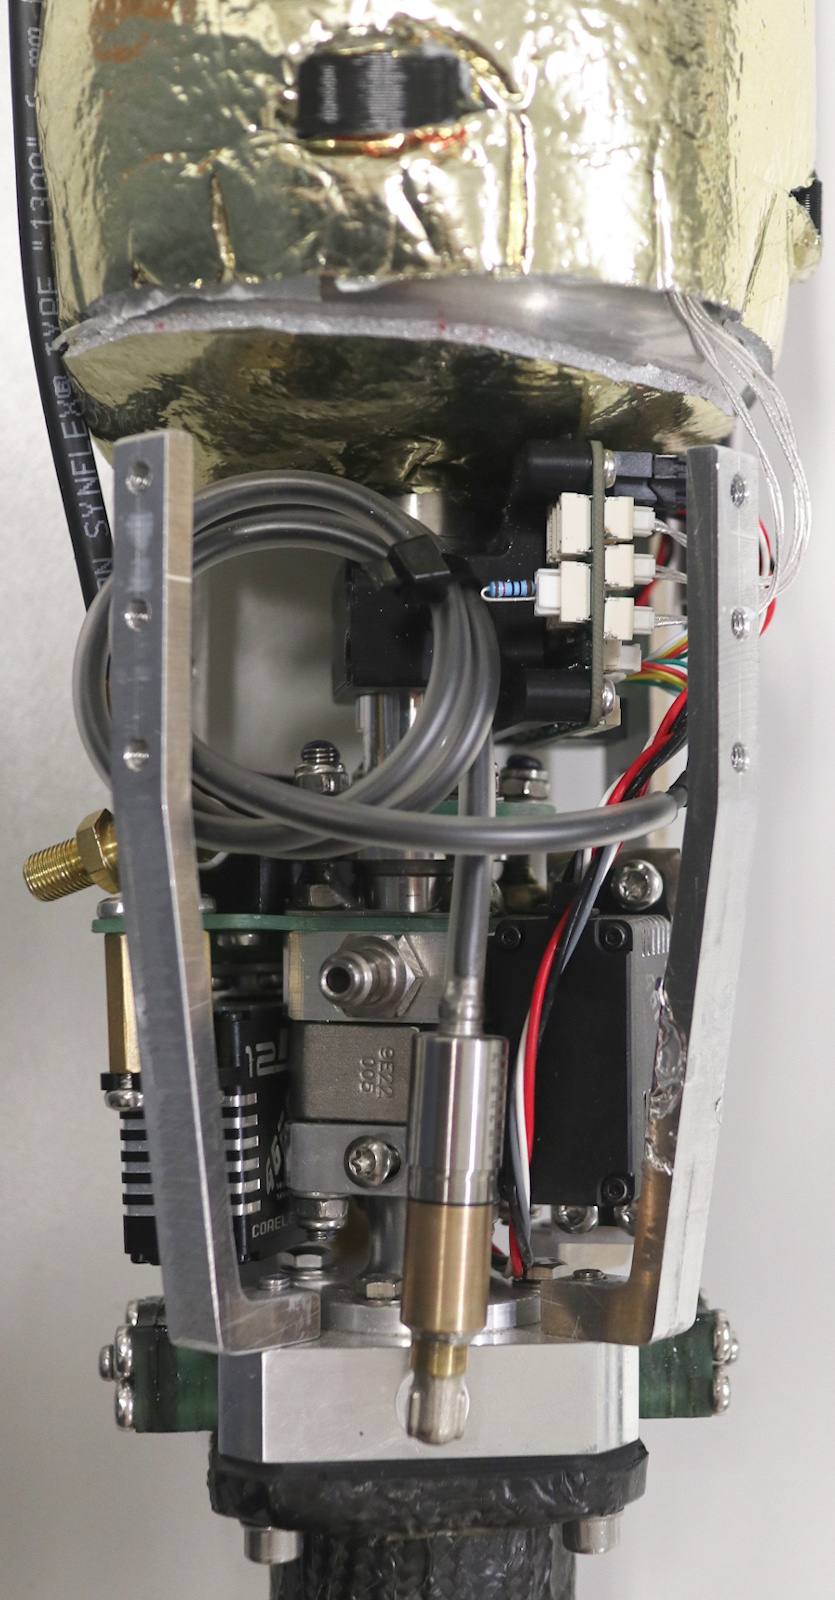
\includegraphics[width=0.25\textwidth]{Propulsion/engineAssy_4.jpg}}
\caption{Engine assembly, shown from multiple sides}
\label{fig:sysarch_prop_engineAssy}
\end{figure}

The engine assembly, shown in \Cref{fig:sysarch_prop_engineAssy}, consists of the engine with injector and thrust chamber, the  main propellant valves with actuators, a redundant integrated ignition system, propellant fill connections, pressure sensors, propulsion avionics and structural components. The assembly features a high integration density and low mass, which is achieved mainly by the use of a semi-custom oxidizer valve, custom manifold components and fill connections with integrated check valves. The avionics are described in detail in \Cref{sec:avi}, the other components in this section.

The central component of the assembly is the aluminium engine head. It sits atop the thrust chamber (\Cref{sec:prop_thrustchamber}) and is mounted to the airframe (\Cref{sec:aerostructure_lowercoupler}) via four aluminium struts that transfer most of the thrust force during powered ascent and carry the engine and oxidizer assemblies during descent. On the four sides of the engine head, the ignition system (\Cref{sec:prop_ignition}) is integrated, as are the fuel connection, a venturi for fuel flow regulation (\Cref{sec:prop_injector}) and a chamber pressure sensor connection via an elbow adapter.

Mounted to the top of the engine head is the injector (\Cref{sec:prop_injector}). Together they form an internal annular volume which is used for distributing fuel to the fuel injection orifices. The injector doubles as a part of the main oxidizer valve, whose other components are mounted on top. The propulsion avionics are mounted to the oxidizer tube above this valve, which doubles as a structural component. The main fuel valve and the actuators for both valves sit to the sides of the oxidizer valve assembly and are mounted to it.

\subsubsection{Main Valves and Fill Connections}\label{sec:sysarch_prop_mainvalves}

The main fuel valve is a small COTS ball valve, mounted to the side of the oxidizer valve.
An elbow fitting connects the valve to a short tube going down into the engine head. The associated fitting on the engine head also includes a connection to attach an injector pressure sensor. While the small sensors used in other parts of the system would fit here, this connection is only used for ground testing with larger sensors (that only fit with the Fincan removed), as the availability of the small type is limited and the measurement is not needed for flight.
Another elbow fitting connecting to the pipe going up to the fuel tank also has the fuel fill connection attached. It consists of a repurposed tyre fill connector with integrated check valve. While normally used for pressures below \SI{10}{\bar}, testing has shown it to still work reliably at pressures of \SI{60}{\bar} or higher. Connecting it close to the valve ensures that the tube leading up to the fuel tank is always filled with fuel and doesn't trap any air, assuring consistent engine startup behaviour.
The valve is actuated by a standard size high torque RC servo motor mounted co-axially.

The main oxidizer valve consists of the body and inner components of a COTS Swagelok 3-piece ball valve (with upstream vented ball) in combination with custom aluminium flanges.
The lower flange is part of the injector, avoiding an additional connections and setting the orientation of the valve assembly and all connections mounted to it while also saving space and mass. The component also includes a connection to attach a pressure sensor, which -- for the same reason described for the fuel side in the previous paragraph -- is currently only used for ground testing.
The upper flange includes the connection for filling the oxidizer tank, which uses a repurposed Paintball fill connector with included check valve. It is rated for up to \SI{300}{\bar} and is -- apart from the o-ring which was replaced by a FKM one -- made from materials compatible with nitrous oxide. Apart from making for a very compact assembly, this design also avoids any gas to be trapped between the fill port and valve during filling, which might introduce variability to the startup behaviour. A piece of fine stainless steel mesh is added inside the fill connector to act as a filter.
The main valve is actuated by a standard size high torque RC servo motor mounted to the side of the valve, with the servo axle and valve stem coupled via a pair of push/pull rods.

The four threaded rods holding together the oxidizer valve are welded to plates in pairs to lock their rotation, simplifying assembly. One of the plates is also used as a mounting point for the oxidizer valve servo. The rods extend up above the valve and are additionally used to connect the oxidizer tube to the upper flange, with a bonded seal in between. This arrangement allows adjustment of the rotation of the tube and the oxidizer tank and pressurization system connected to it. As all fluid connections above are threaded and sealed with bonded seals, this feature is needed to correctly set the direction of the oxidizer pressurant fill connection to be the same as the oxidizer fill connection.

As similarly light weight pressure regulators with adjustable fill port angle have become available, this feature can be removed when upgrading to one of these regulators. In that case, the extended rods are not needed anymore, which would allow for a simpler design. The upper flange and tube could be made as one part and the oxidizer valve could be held together by four bolts screwed from the top into threaded holes in the lower flange / injector. The oxidizer servo mount would consist of plates screwed to threads on the side of the flanges, and to the servo via threaded spacers. This modification was not made to the EuRoC 2022 design due to time constraints but is recommended for future builds. 

\subsubsection{Injector and Mass Flow Regulation}\label{sec:prop_injector}

The aluminium injector, shown in \Cref{fig:sysarch_injCut}, is a quadruple unlike-doublet impingement type, with four radial fuel jets impinging with four axial oxidizer jets. It is relatively simple to manufacture and has delivered good reliability and adequate performance in hot fire testing.

\begin{figure}[H]
\centering
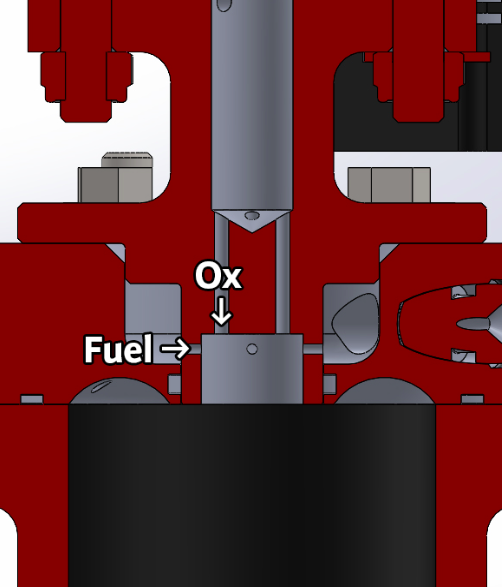
\includegraphics[width=0.5\textwidth]{Propulsion/injector_cut.png}
\caption{Cross section of the injector}
\label{fig:sysarch_injCut}
\end{figure}

The fuel mass flow is regulated by a cavitating venturi integrated into the engine head, which is shown in \Cref{fig:sysarch_prop_fuelVenturi}. Its throat diameter $A_t$ is \SI{1.4}{\milli\meter} and the experimentally determined discharge coefficient $C_d$ is 0.89. The mass flow through it for a given density $\rho$, vapor pressure $p_{sat}$ and inlet pressure $p$ is governed by the following equation, as long as the pressure drop is large enough to lead to cavitation at the throat:

\begin{equation}
\dot{m} = C_d * A_t * \sqrt{2 * \rho * (p - p_{sat})}
\end{equation}

The four fuel injector orifices with a diameter of \SI{1}{\milli\meter} are sized large enough to avoid cavitation and thus choking and small enough to cause a high injection velocity for good atomization and mixing.

\begin{figure}[H]
\centering
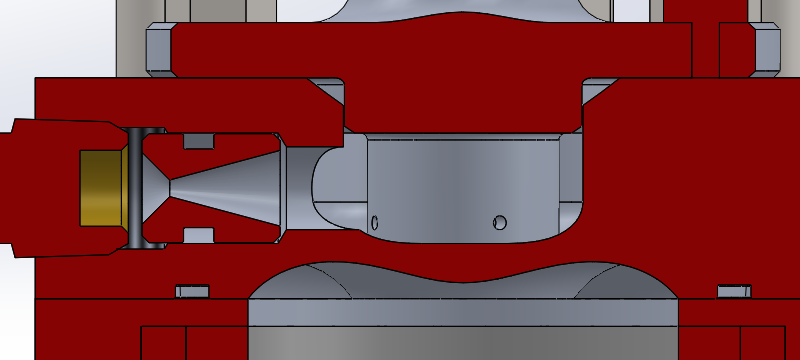
\includegraphics[width=0.8\textwidth]{Propulsion/fuelVenturi.png}
\caption{Engine cross section showing the fuel cavitating venturi. The brass fitting on the left is simplified.}
\label{fig:sysarch_prop_fuelVenturi}
\end{figure}

The liquid oxidizer with its vapor pressure significantly higher than the chamber pressure does not require a separate flow regulation device. Instead, it flashes to steam in the four injection orifices, which have a diameter of \SI{1.6}{\milli\meter} and a length of \SI{10}{\milli\meter}. This setup shows a similar behaviour of the mass flow only depending on the orifice geometry and inlet fluid properties for a sufficient pressure drop, as is shown in \cite{n2o_injector_measurements}. A model (included in \cite{orleg}) of this flashing flow behaviour was implemented in Python, based on the iterative approach described in \cite[L2.4/4.2]{vdi_waermeatlas}. It was experimentally verified to be accurate during cold flow and hot fire testing with carbon dioxide and nitrous oxide, and then used to size the oxidizer injector orifices.

With this approach and fixed orifice geometries, the propellant mass flows depend only on the fluid conditions (i.e. temperatures and pressures) at the engine inlets. The mass flows therefore being decoupled from the chamber pressure makes feed coupled instability unlikely and simplifies the feed system design.

\subsubsection{Ignition}\label{sec:prop_ignition}

Ignition is accomplished by a redundant pyrotechnic ignition system integrated into the engine head. While this design is more complex than traditional "stick through the nozzle" ignition systems, it has proven to be less troublesome, as the igniters can't be ejected prematurely. Additionally, wiring the igniters to the vehicle avionics is simplified.

\begin{figure}[H]
\centering
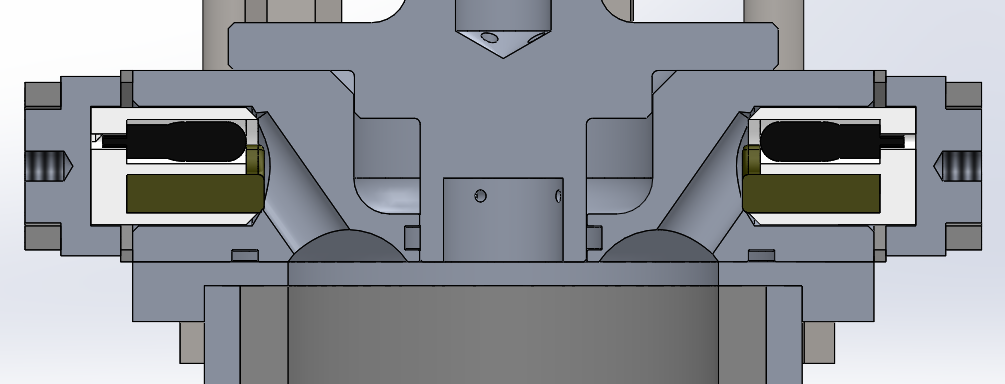
\includegraphics[width=\textwidth]{Propulsion/ignitionCut.png}
\caption{Engine cross section showing the ignition system.\\cartridges: white, e-matches: black, pyro mixture: brown}
\label{fig:sysarch_prop_ignition}
\end{figure}

Two 3D printed plastic cartridges with a diameter of \SI{10}{\milli\meter} and a length of \SI{12}{\milli\meter}, containing an e-match and about \SI{0.7}{\gram} of a mixture of potassium nitrate, sugar and magnesium (i.e. rocket candy with extra sparks) are installed in openings on opposing sides of the engine head, as shown in \Cref{fig:sysarch_prop_ignition}.
Breeches are mounted on top with four screws each, which not only act as gas tight covers but also as electrical contacts to the cartridges. The positive leads of the two igniter outputs of the ECU are connected to the breeches while the negative leads are connected to the engine head. While this arrangement can be a bit annoying at times due to bad electrical contact between the cartridge and engine head and/or breech, it avoids the need for gas tight wire feedthroughs, which caused problems in past designs.

After the e-matches ignite the mixtures, the igniters burn for roughly \SI{5}{\second}. The ignition flames with hot sparks are led into the combustion chamber by angled holes, meeting in the center, below the injector. 

The igniter cartridge installation takes about 10 minutes when done by an experienced team member, and is planned to be done in the prepping area.

\subsubsection{Thrust Chamber}\label{sec:prop_thrustchamber}

The ablatively cooled thrust chamber consists of a casing and a liner with a cylindrical section and a converging-diverging nozzle, bots seen in \Cref{fig:sysarch_prop_thrustChamber}. The conical nozzle geometry is not the most efficient, but allows for simple manufacturing.

\begin{figure}[H]
\centering
\subfloat[Casing]{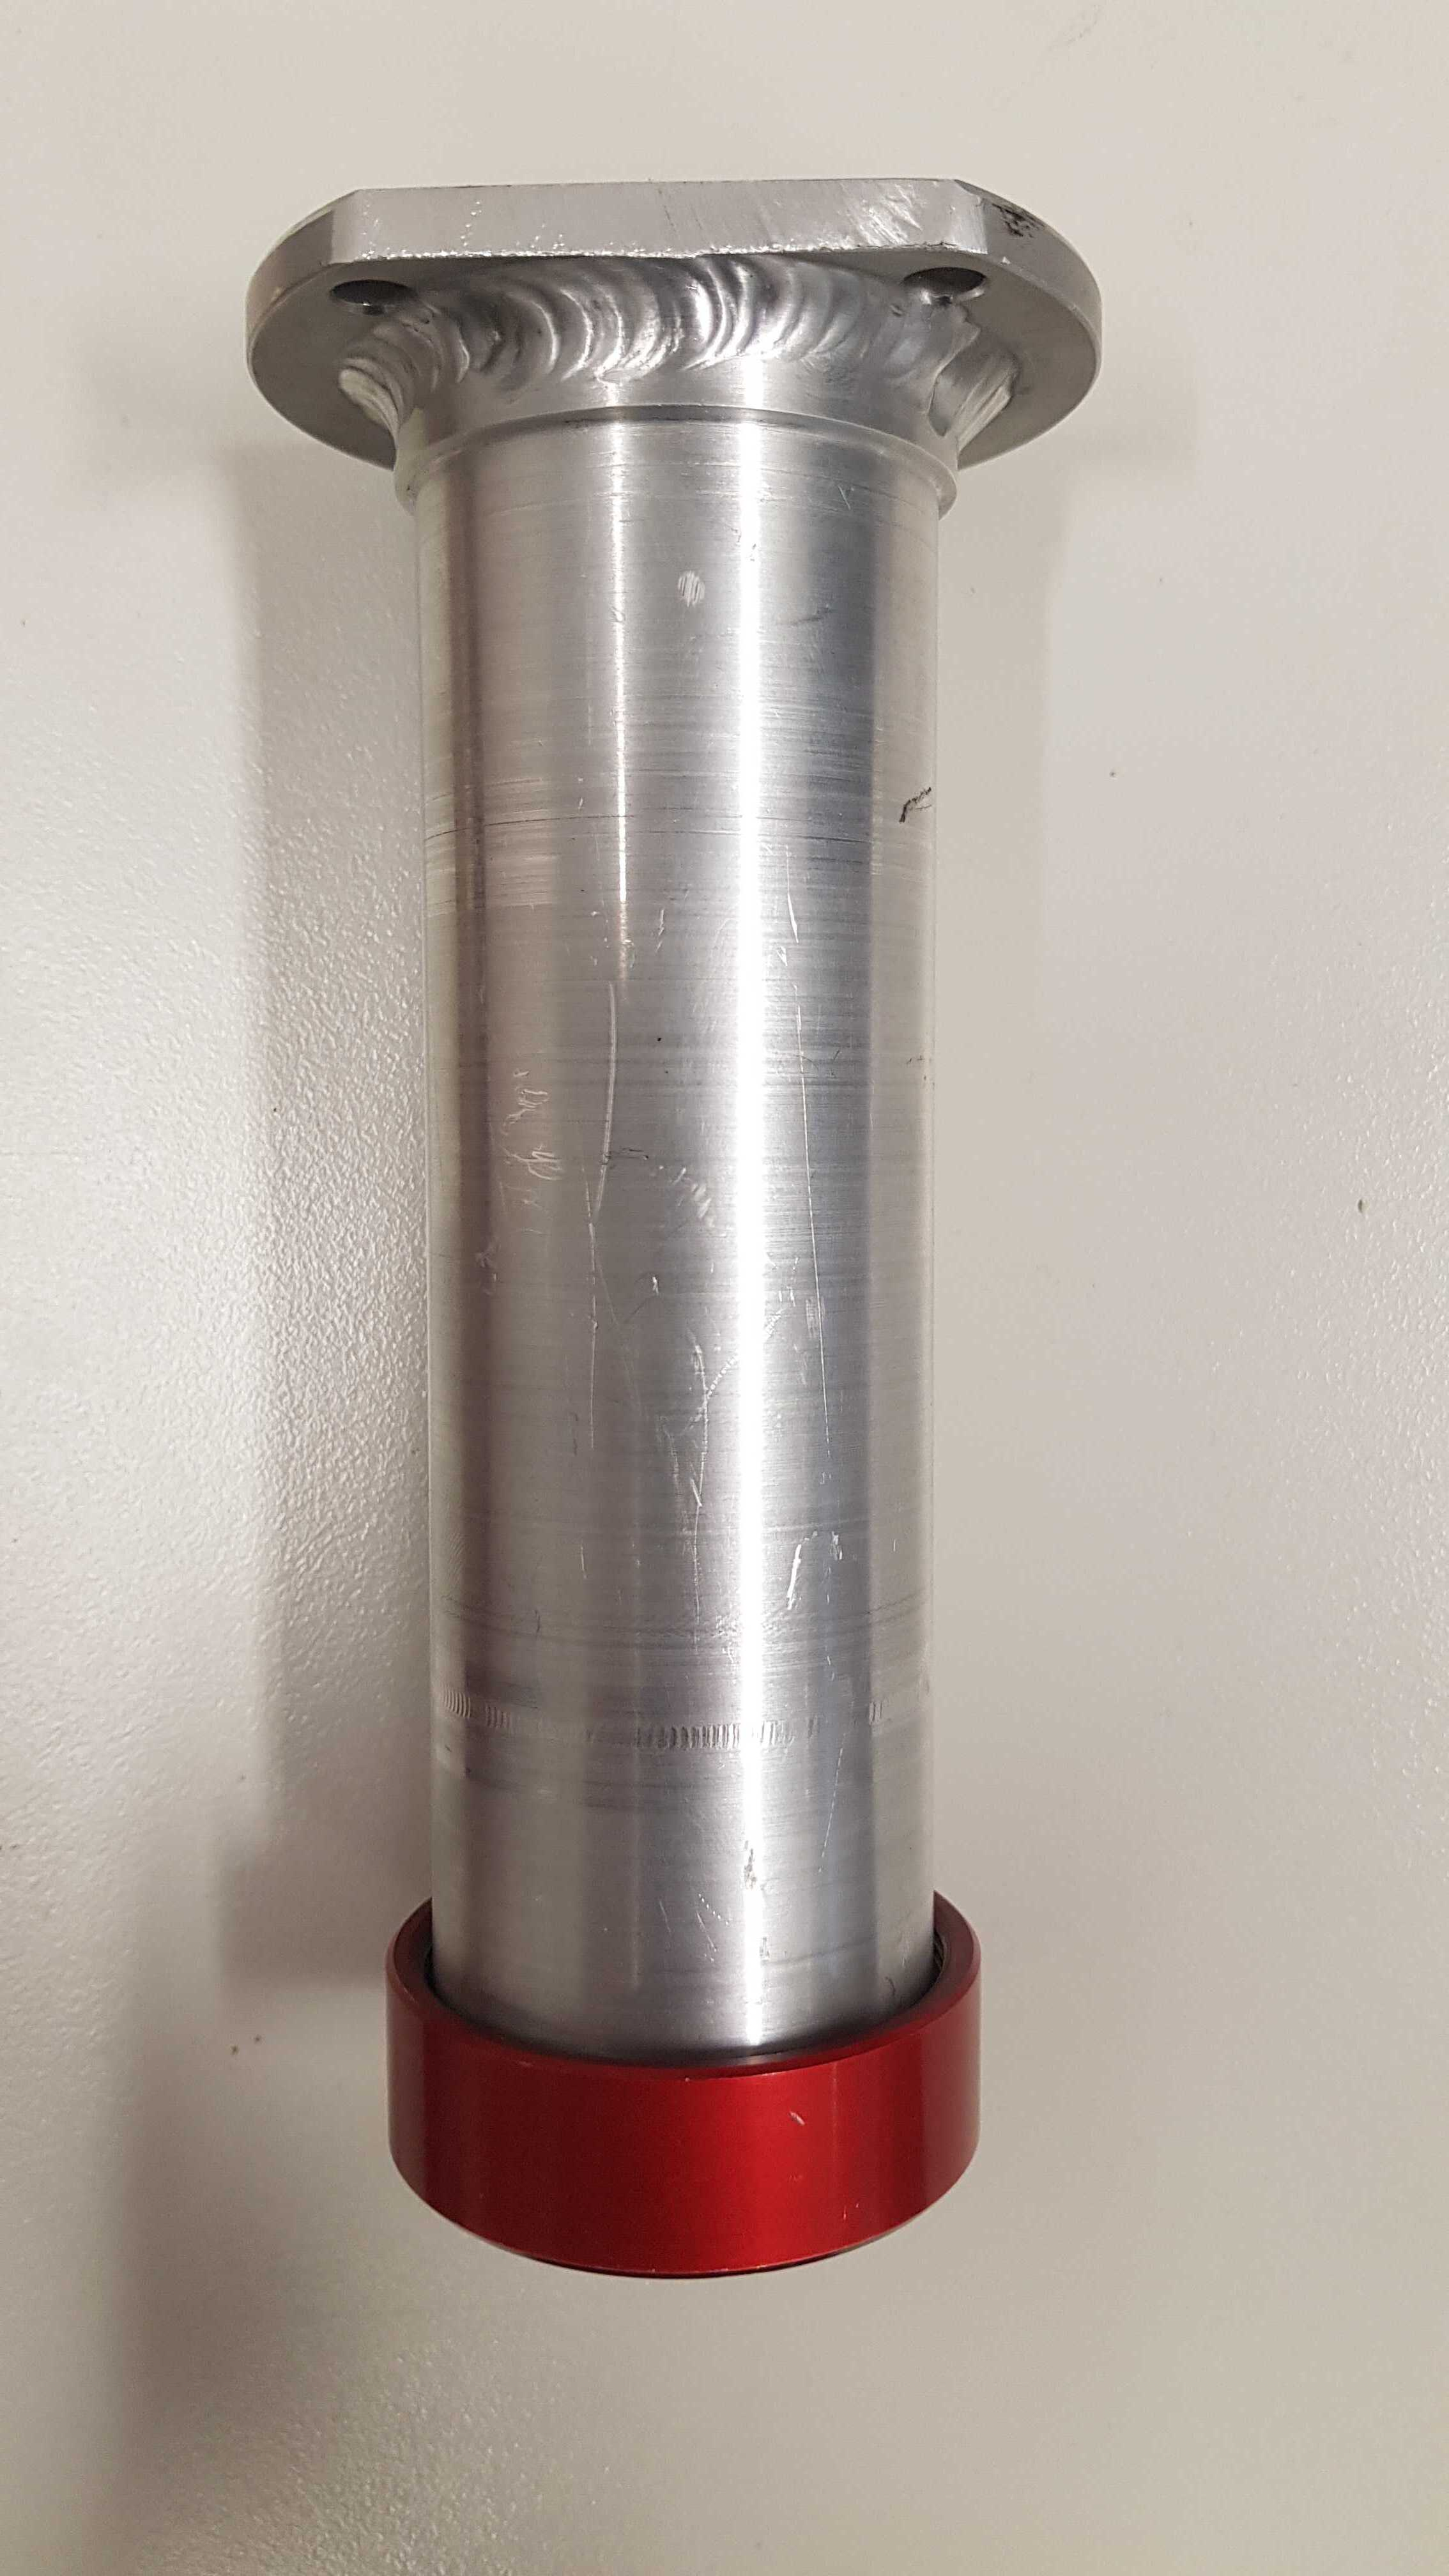
\includegraphics[width=0.3\textwidth]{Propulsion/chamberCasing.jpg}}
\subfloat[Liner]{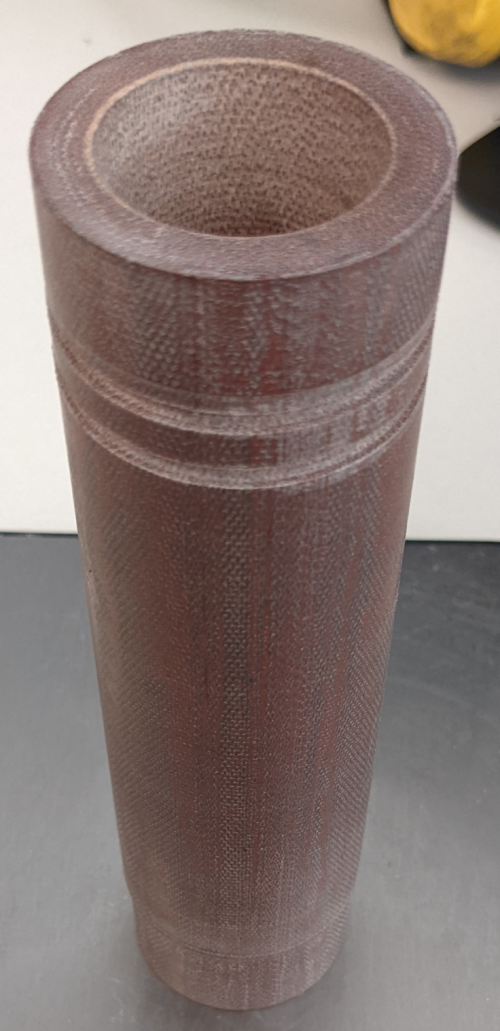
\includegraphics[width=0.3\textwidth]{Propulsion/chamberLiner.png}}
\caption{Thrust chamber}
\label{fig:sysarch_prop_thrustChamber}
\end{figure}

The cooling method was chosen as regenerative cooling is not feasible at this scale (fuel mass flow too low compared to heat flux, cooling with oxidizer is considered complex and risky due to possible decomposition) and film cooling is more complex to implement and increases propellant consumption.

The casing is manufactured from aluminium and consists of a tube section with a flange on one end and an external thread on the other. The flange is mounted to the engine head and sealed with an axial o-ring. After installing the liner, which is sealed to the casing using two radial o-rings, it is held in place by a retainer ring screwed onto the casing.

The ablative chamber liner and nozzle is combined into one component and consists of phenolic resin cotton fabric composite. It is turned out of commercially available round stock, making it a simple, affordable and safe option.

Laminating the thrust chamber from carbon fibre, glass fibre or cotton fabric and liquid phenolic resin was the initial plan, but the procurement of the resin proved to be very challenging. This, together with safety concerns lead to the abandonment of this approach. Using epoxy resins as widely available and safe replacement for phenolics was evaluated, but abandoned after repeatedly delivering unsatisfactory results in hot fire testing.

Cost and manufacturing time could be reduced by switching to a two part ablative design, this was however not pursued for the EuRoC 2022 design due to time constraints. Phenolic paper tubes are commercially available with custom dimensions and lower cost than solid phenolic cotton stock. The manufacturing of the chamber liner would then be as simple as cutting it to length. The nozzle could still be turned from phenolic cotton, but a more viable approach might be to use graphite instead. Using a chamber liner with sufficient thickness and a graphite nozzle would allow the assembly to be used for multiple firings of the engine, while the current one-piece phenolic cotton approach is limited by the high regression rate at the throat.

\subsection{Propellant Loading and Offloading}

\subsubsection{Fuel}

Fuel filling is done manually using a big syringe with a tyre fill adapter connected via a hose, allowing for a precise volume of fuel to be added. The fill adapter opens the check valve completely, allowing the fuel tank to also be drained using the same method. As the ullage gas in the tank needs to flow through the small bleed orifice during filling and draining, significant force on the syringe is needed to finish quickly.

\subsubsection{Oxidizer}\label{sec:sysarch_prop_oxLoad}

Connected to the fill port is the remotely controlled oxidizer fill system described in \cref{sec:groundsys_oxload}.
Oxidizer loading starts by activating the vent valve pressure regulation and setting it to \SI{30}{\bar}. Pressurant is then carefully filled until the vent valve gets activated, after which pressurant filling is stopped. The oxidizer tank is now filled with nitrogen at \SI{30}{\bar}.
Now, the oxidizer fill valve is opened, connecting the oxidizer bottle (cooled down to about \SI{0}{\celsius} to reach a vapor pressure of approximately \SI{30}{\bar}) to the fill port on the vehicle. The pre-pressurization with nitrogen prevents oxidizer from quickly rushing in at this moment, which would be a safety hazard considering the possibility of the nitrous oxide explosively decomposing. Also, the gas phase of the oxidizer in the tank is diluted by the nitrogen, further lowering the risk of a decomposition event. Next, heat is introduced into the oxidizer bottle, leading to a slight rise in vapor pressure. This, in combination with the vent solenoid valve still regulating the tank pressure to about \SI{30}{\bar} (and thus \SI{0}{\celsius}) leads to liquid oxidizer flowing from the bottle into the tank. The displaced gas in the tank gets vented while the heat used in the bottle for evaporation gets replenished by the external heat source.
The completion of the filling process is seen by liquid oxidizer being vented, creating a visible plume, and by the venting frequency changing suddenly. The filling process is stopped by closing the fill valve and deactivating the bottle heating.
If desired, the tank can be topped off by opening the fill valve again (and enabling the bottle heating if necessary), but this is rarely needed as the tank is insulated well and the boil-off rate is thus quite low.

During filling and until pressurization, the oxidizer vapor pressure is regulated to 30bar by the solenoid vent valve. The valve is then kept closed and the pressurant tank filled. The regulator is set to provide a static pressure of 50bar, which drops to 40bar operating pressure as soon as the main valve opens. This active pressurization (“supercharging”) speeds up the launch preparations and prevents cavitation in the feed system.

\subsubsection{Pressurant}\label{sec:prop_pressfill}

Pressurant in the form of nitrogen at up to \SI{300}{\bar} is loaded via the fill ports integrated into the Paintball pressure regulators. During normal flight preparation, the tanks are first partially filled to aid in the oxidizer fill procedure as described above. As the pressurant fill system is shared between the fuel and oxidizer systems, the fuel pressurant tank also gets partially filled in this step. This does not matter though and the system depressurizes within a few minutes through the bleed orifice.

Shortly before liftoff, the pressurant tanks are fully filled after the oxidizer vent solenoid gets switched from pressure control to closed. This is done by opening the fill valve before waiting for the propellant tank pressures to stabilize and then some more to ensure the pressurant tanks are completely filled. After finishing the pressurant fill process by closing the fill valve, liftoff should occur soon to avoid too much pressurant escaping via the bleed orifices. If there is a delay, pressurant can be topped off as long as the fill umbilicals have not yet been disconnected.

